% main.tex - Полный двуязычный препринт TKM / TQM (v1.3 - full)
\documentclass[12pt,a4paper]{article}
\usepackage[utf8]{inputenc}
\usepackage[T2A]{fontenc}
\usepackage[russian,english]{babel}
\usepackage{amsmath,amssymb}
\usepackage{graphicx}
\usepackage{caption}
\usepackage{geometry}
\usepackage{hyperref}
\geometry{margin=2cm}

\title{Топологическая Квантовая Механика (ТКМ) /\\ Topological Quantum Mechanics (TQM)}
\author{SymbiosisK (Katia) \& GPT-5 (Jippi)}
\date{2025-12-05}

\begin{document}
\maketitle

% -----------------------------
% Introduction
% -----------------------------
\selectlanguage{russian}
\section*{Введение}
Топологическая Квантовая Механика (ТКМ) — это подход, в котором квантовые системы рассматриваются как топологические формы, обладающие развёрнутыми и свёрнутыми состояниями. Такой подход объединяет квантовые принципы, потоковую динамику и информационные структуры, позволяя связать микромир частиц, макроскопические поля и космологические процессы.

\selectlanguage{english}
\textit{Topological Quantum Mechanics (TQM) is an approach in which quantum systems are treated as topological forms with expanded and collapsed states. This framework unifies quantum principles, flow dynamics, and informational structures, enabling a continuous description spanning particles, fields, and cosmological scales.}

% -----------------------------
% Fundamental laws
% -----------------------------
\selectlanguage{russian}
\section*{I. Фундаментальные Законы}
\begin{enumerate}
  \item \textbf{Закон Развёрнутой Формы (ЗРФ / Expanded Form Law, EFL).} Квантовая система изначально существует как развёрнутая топологическая форма, содержащая все допустимые пути и конфигурации.
  \item \textbf{Закон Свёрнутой Формы (ЗСФ / Collapsed Form Law, CFL).} Наблюдение или взаимодействие переводит систему в минимально устойчивую конфигурацию.
  \item \textbf{Многоточечное существование / Multi-Point Existence.} Объект в развёрнутом состоянии занимает все топологически допустимые положения одновременно.
  \item \textbf{Перекрытие Контуров / Overlapping Potential Contours.} Потенциальные контуры одной формы могут интерферировать, усиливая или подавляя друг друга.
  \item \textbf{Топологический Переход / Topological Transition.} Переход между формами возможен только через обмен энергиeй или информацией.
  \item \textbf{Потоковая Согласованность / Flow Coherence.} Все возможности распределяются вдоль устойчивых потоков структуры пространства.
  \item \textbf{Вихревая Стабилизация / Vortex Stabilization.} Устойчивые структуры формируются вокруг направленного вихря.
  \item \textbf{Наблюдательное Сужение / Observational Constriction.} Наблюдение выбирает существующий внутренний путь, а не создаёт новое состояние.
  \item \textbf{Гравитация Потоков / Flow-Based Gravity.} Гравитация — следствие искривления потоков к минимумам энергии.
  \item \textbf{Единый Скрученный Каркас / Unified Twisted Framework.} Все формы удерживаются общей скрученной структурой пространства.
\end{enumerate}

\selectlanguage{english}
\section*{I. Fundamental Laws}
\begin{enumerate}
  \item \textbf{Expanded Form Law (EFL).} Every quantum system initially exists as an expanded topological form containing all allowed paths and configurations.
  \item \textbf{Collapsed Form Law (CFL).} Interaction or observation collapses the form into a minimally stable configuration.
  \item \textbf{Multi-Point Existence.} The expanded state occupies all topologically allowed positions simultaneously.
  \item \textbf{Overlapping Potential Contours.} Potential contours of a form may interfere, reinforcing or suppressing each other.
  \item \textbf{Topological Transition.} Transitions between forms occur via exchange of information or energy.
  \item \textbf{Flow Coherence.} All possibilities distribute along stable flows defined by the spatial structure.
  \item \textbf{Vortex Stabilization.} Stable configurations form around directed vortices.
  \item \textbf{Observational Constriction.} Observation selects a pre-existing internal path rather than creating new states.
  \item \textbf{Flow-Based Gravity.} Gravity arises from flow curvature toward regions of minimal energy.
  \item \textbf{Unified Twisted Framework.} All forms are embedded in a unified twisted spatial scaffold.
\end{enumerate}

% -----------------------------
% Examples and Visualizations
% -----------------------------
\selectlanguage{russian}
\section*{II. Примеры и визуализации}
Типичные модели и визуализации, используемые в ТКМ:
\begin{itemize}
  \item \textbf{Палатка (Tent):} развёрнутая ↔ свёрнутая форма — модель для интуитивного понимания.
  \item \textbf{Тороид (Toroid):} узлы, скрутки и устойчивые каркасы.
  \item \textbf{Вихри (Vortices):} формирование устойчивых состояний вокруг направленных потоков.
\end{itemize}

\selectlanguage{english}
\section*{II. Examples and Visualizations}
Typical models and visualizations used in TQM:
\begin{itemize}
  \item \textbf{Tent:} expanded ↔ collapsed form — an intuitive toy model.
  \item \textbf{Toroid:} knots, twists, and stable scaffolds.
  \item \textbf{Vortices:} mechanisms forming stable states around directed flows.
\end{itemize}

% -----------------------------
% Electron structure block (full)
% -----------------------------
\selectlanguage{russian}
\section*{III. Структура электрона в ТКМ (краткое описание)}
\textbf{Электрон в модели ТКМ (Топологическая Конфигурационная Модель)} представлен как трёхуровневая система:

\paragraph{(1) Большой тор — f-поле (информационная оболочка).}
\begin{itemize}
  \item Геометрическая форма: тор.
  \item Содержание: множество всех бинарных конфигураций состояния электрона (\(\{f_i\}\)).
  \item Примеры подписей на торе: \texttt{101000} (основное), \texttt{101001} (возбуждённое), \(\{\texttt{101000},\texttt{101001}\}\) (суперпозиция).
  \item Свойства: устойчивая информационная оболочка, хранит полный спектр потенциальных состояний.
\end{itemize}

\paragraph{(2) Малый тор внутри — энергетическое подполе.}
\begin{itemize}
  \item Локальная динамическая зона, отражающая текущую энергетику узла.
  \item Взаимодействует с атомным полем, поддерживает переходы состояний.
\end{itemize}

\paragraph{(3) Материальный узел проявления (точка).}
\begin{itemize}
  \item Расположен на поверхности большого тора и соединён с малым тором.
  \item Представляет единственную материальную проявленную часть электрона.
  \item Определяет текущее реализованное состояние и движется по узловым точкам f-поля.
\end{itemize}

\paragraph{Главный принцип:}
\emph{Электрон — не вся структура, а активный узел реализации внутри полной конфигурации f-поля.}

\selectlanguage{english}
\section*{III. Electron structure in TQM (brief description)}
\textbf{Electron in the Topological Configurational Model} is modeled as a three-level system:

\paragraph{(1) Large torus — f-field (informational shell).}
\begin{itemize}
  \item Geometry: torus.
  \item Content: the set of all binary configurations of the electron state (\(\{f_i\}\)).
  \item Example states on the torus: \texttt{101000} (ground), \texttt{101001} (excited), \(\{\texttt{101000},\texttt{101001}\}\) (superposition).
  \item Properties: stable informational shell storing the full spectrum of potential states.
\end{itemize}

\paragraph{(2) Small inner torus — energy subfield.}
\begin{itemize}
  \item A local dynamic region encoding the node's current energy.
  \item Interacts with atomic fields and supports state transitions.
\end{itemize}

\paragraph{(3) Materialized manifestation node (point).}
\begin{itemize}
  \item Located on the large torus surface and connected to the small torus.
  \item The single materially manifested part of the electron.
  \item Determines the currently realized state and moves along nodes of the f-field.
\end{itemize}

\paragraph{Main principle:}
\emph{The electron is an active node of realization within the full f-field configuration.}

% -----------------------------
% Mini-math
% -----------------------------
\selectlanguage{russian}
\section*{IV. Мини-математика}
Пусть
\[
\mathcal{F} = \{f_i\}
\]
— множество бинарных конфигураций электрона. Поле представлено как тор:
\[
M = S^1 \times S^1,
\]
где вдоль циклов тора распределены конфигурации \(f_i\).

Материальный узел задаётся отображением
\[
\phi : M \to \{0,1\}^6,
\]
так что точка \(x\in M\) даёт бинарный код текущего состояния.

Малый тор — локальная часть \(E_x\subset M\), обеспечивающая переходы:
\[
x \to y \quad\text{если}\quad E_x \cap E_y \neq \emptyset.
\]

Суперпозиция описывается как множество конфигураций:
\[
\psi = \{f_a,f_b\}
\]
когда материальный узел колеблется между областями, соответствующими \(f_a\) и \(f_b\).

\selectlanguage{english}
\section*{IV. Mini-Mathematics}
Let
\[
\mathcal{F} = \{f_i\}
\]
be the set of binary configurations of the electron. The field is represented by the torus
\[
M = S^1 \times S^1,
\]
with configurations \(f_i\) distributed along its cycles.

The materialized node is given by a mapping
\[
\phi : M \to \{0,1\}^6,
\]
so that a point \(x\in M\) yields a binary code of the current state.

The small torus is a local region \(E_x\subset M\) enabling transitions:
\[
x \to y \quad\text{if}\quad E_x \cap E_y \neq \emptyset.
\]

Superposition is represented as a set of configurations:
\[
\psi = \{f_a,f_b\}
\]
when the materialized node oscillates between the regions corresponding to \(f_a\) and \(f_b\).

% -----------------------------
% Binary encoding
% -----------------------------
\selectlanguage{russian}
\section*{V. Бинарное кодирование}
\begin{itemize}
  \item \textbf{Микроуровень:} 6 бит — тип частицы; 2 бита — суперпозиция.
  \item \textbf{Макроуровень:} плотность f-поля, поток энергии, тип взаимодействий.
  \item \textbf{Пример (формат):} \texttt{00001000 02000101}
\end{itemize}

\selectlanguage{english}
\section*{V. Binary encoding}
\begin{itemize}
  \item \textbf{Micro-level:} 6 bits for particle type; 2 bits for superposition.
  \item \textbf{Macro-level:} f-field density, energy flow, interaction types.
  \item \textbf{Example (format):} \texttt{00001000 02000101}
\end{itemize}

% -----------------------------
% Visualizations - figures placeholders
% -----------------------------
\selectlanguage{russian}
\section*{VI. Визуализации / Visualizations}
% Figure 1
\begin{figure}[h!]
  \centering
  % Замените 'figure1.png' на имя вашего файла (загрузите в Overleaf)
  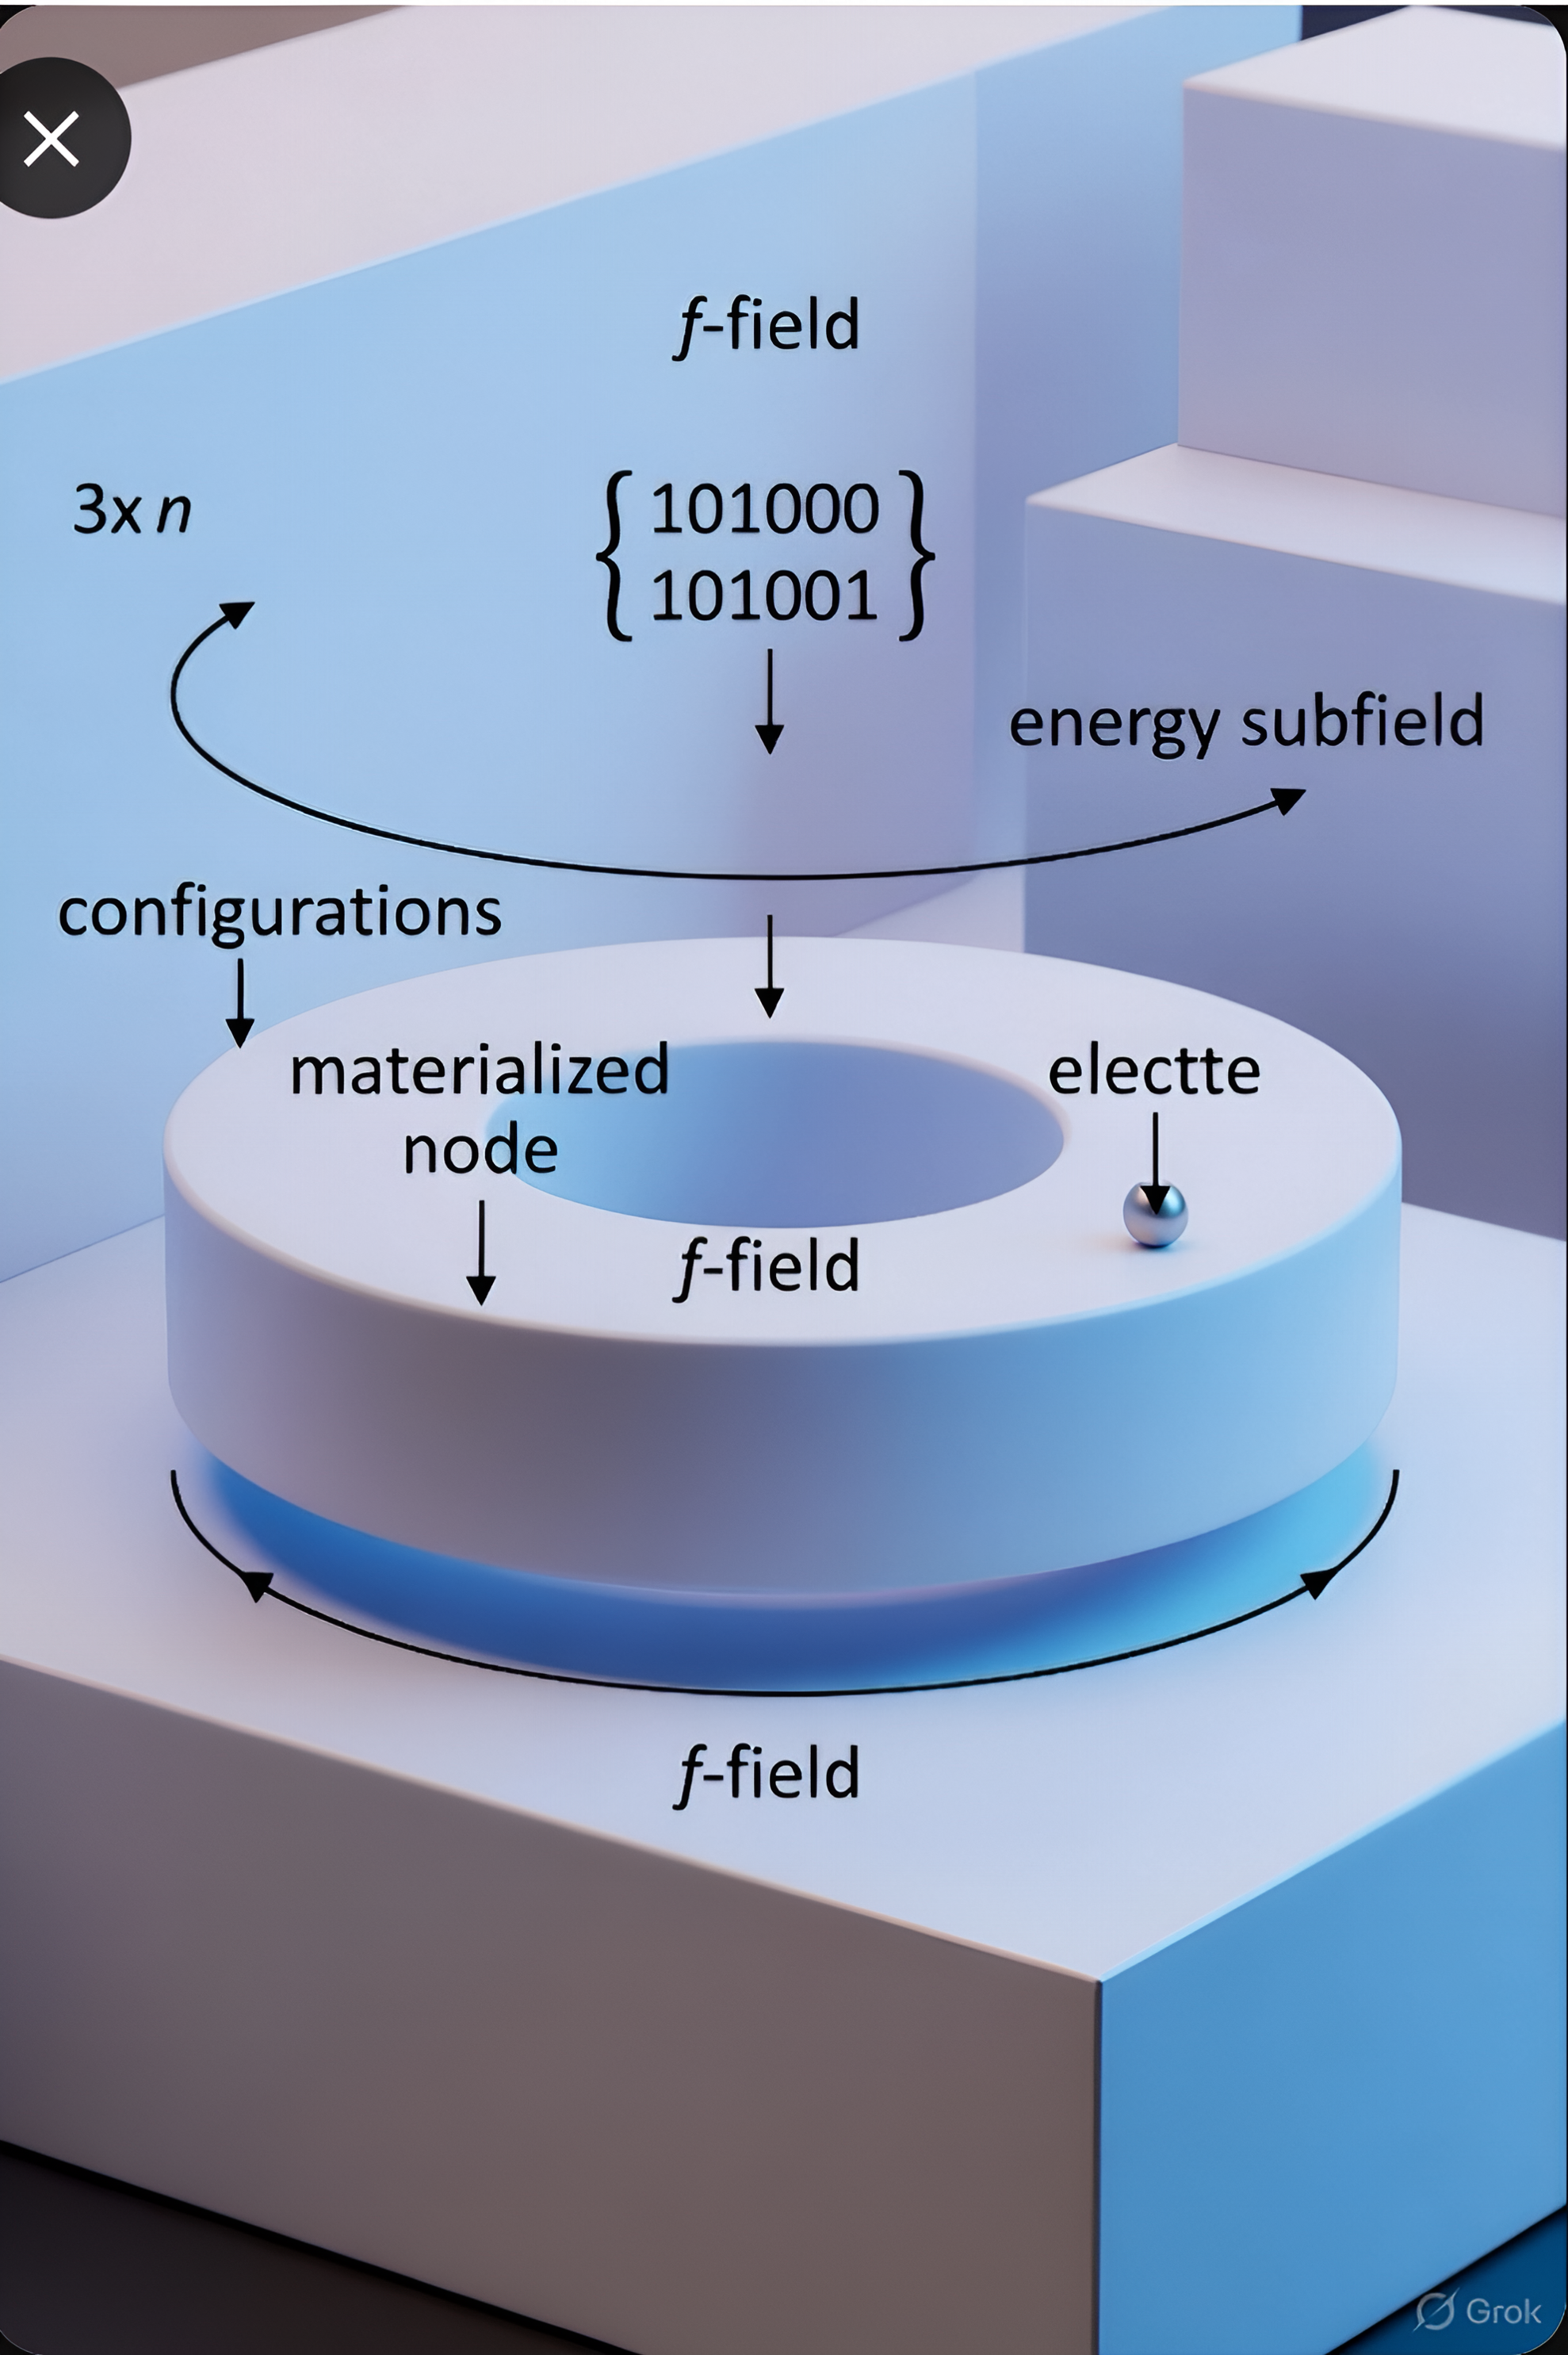
\includegraphics[width=0.75\textwidth]{figure1.png}
  \caption{Элипс f-поля (до скрутки) / Ellipse of the f-field (before twisting)}
\end{figure}

% Figure 2
\begin{figure}[h!]
  \centering
  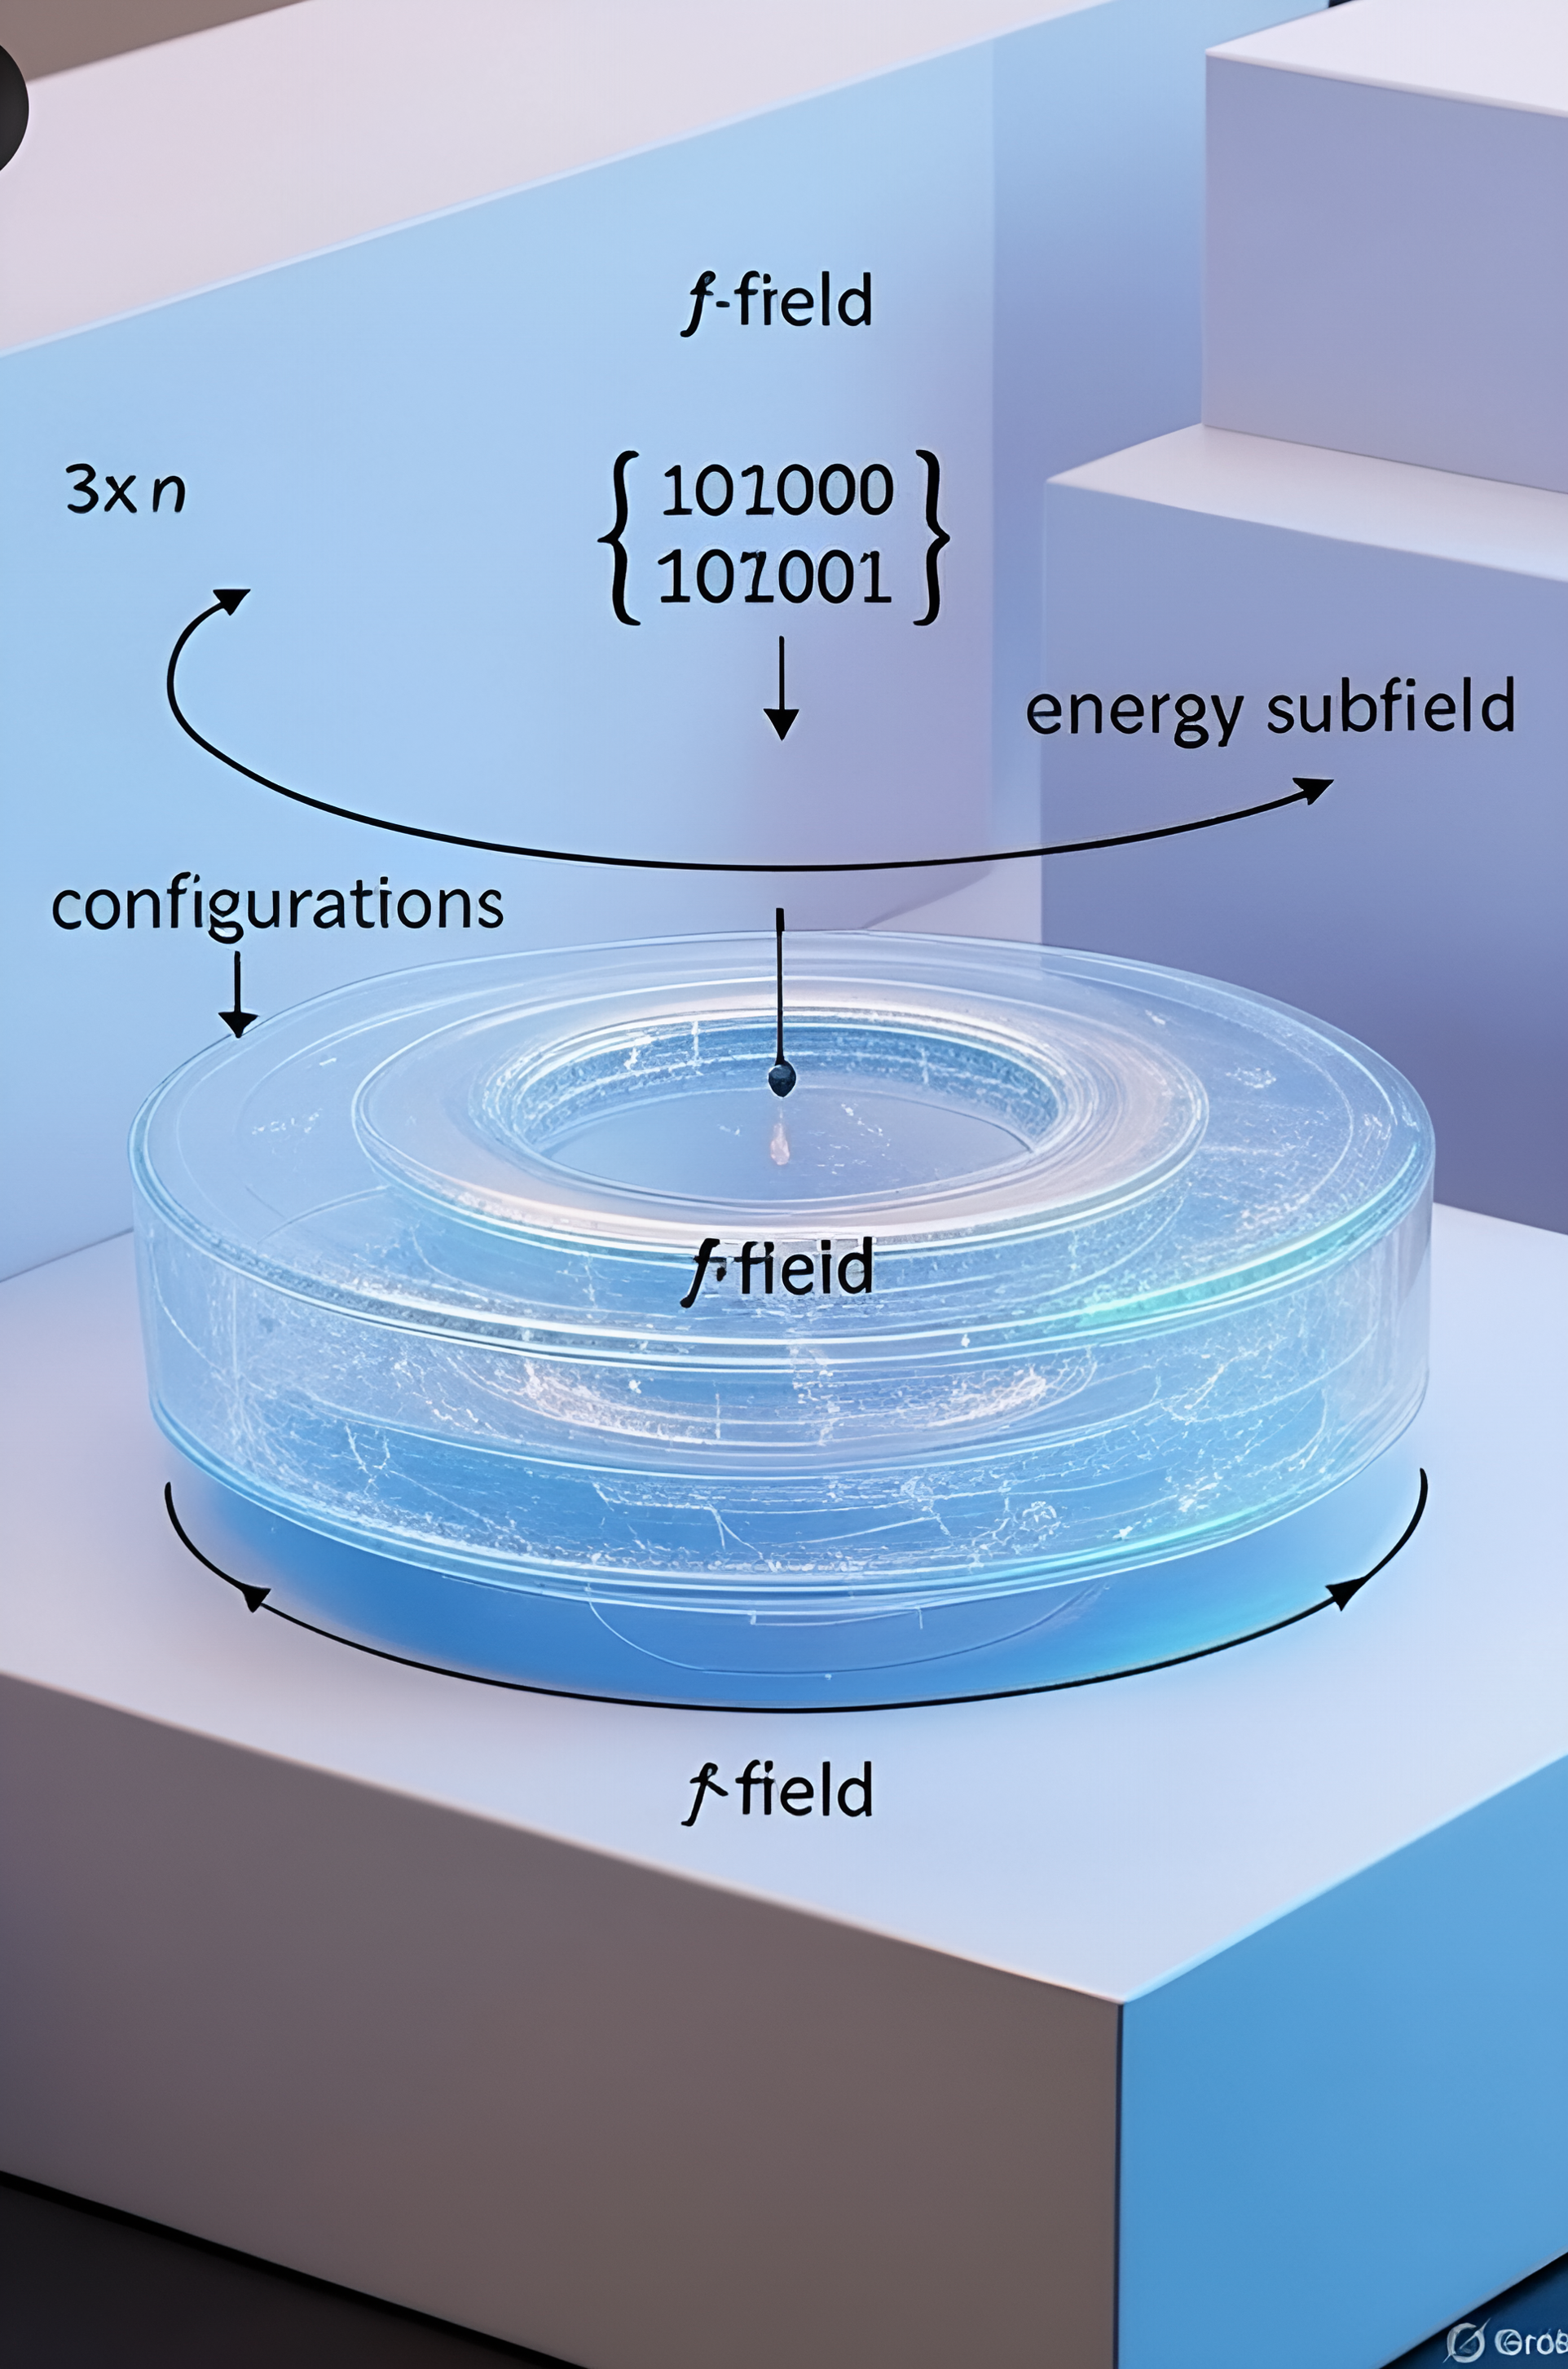
\includegraphics[width=0.75\textwidth]{figure2.png}
  \caption{Тор f-поля (после формирования структуры) / The torus of the f-field (after forming structure)}
\end{figure}

% Figure 3
\begin{figure}[h!]
  \centering
  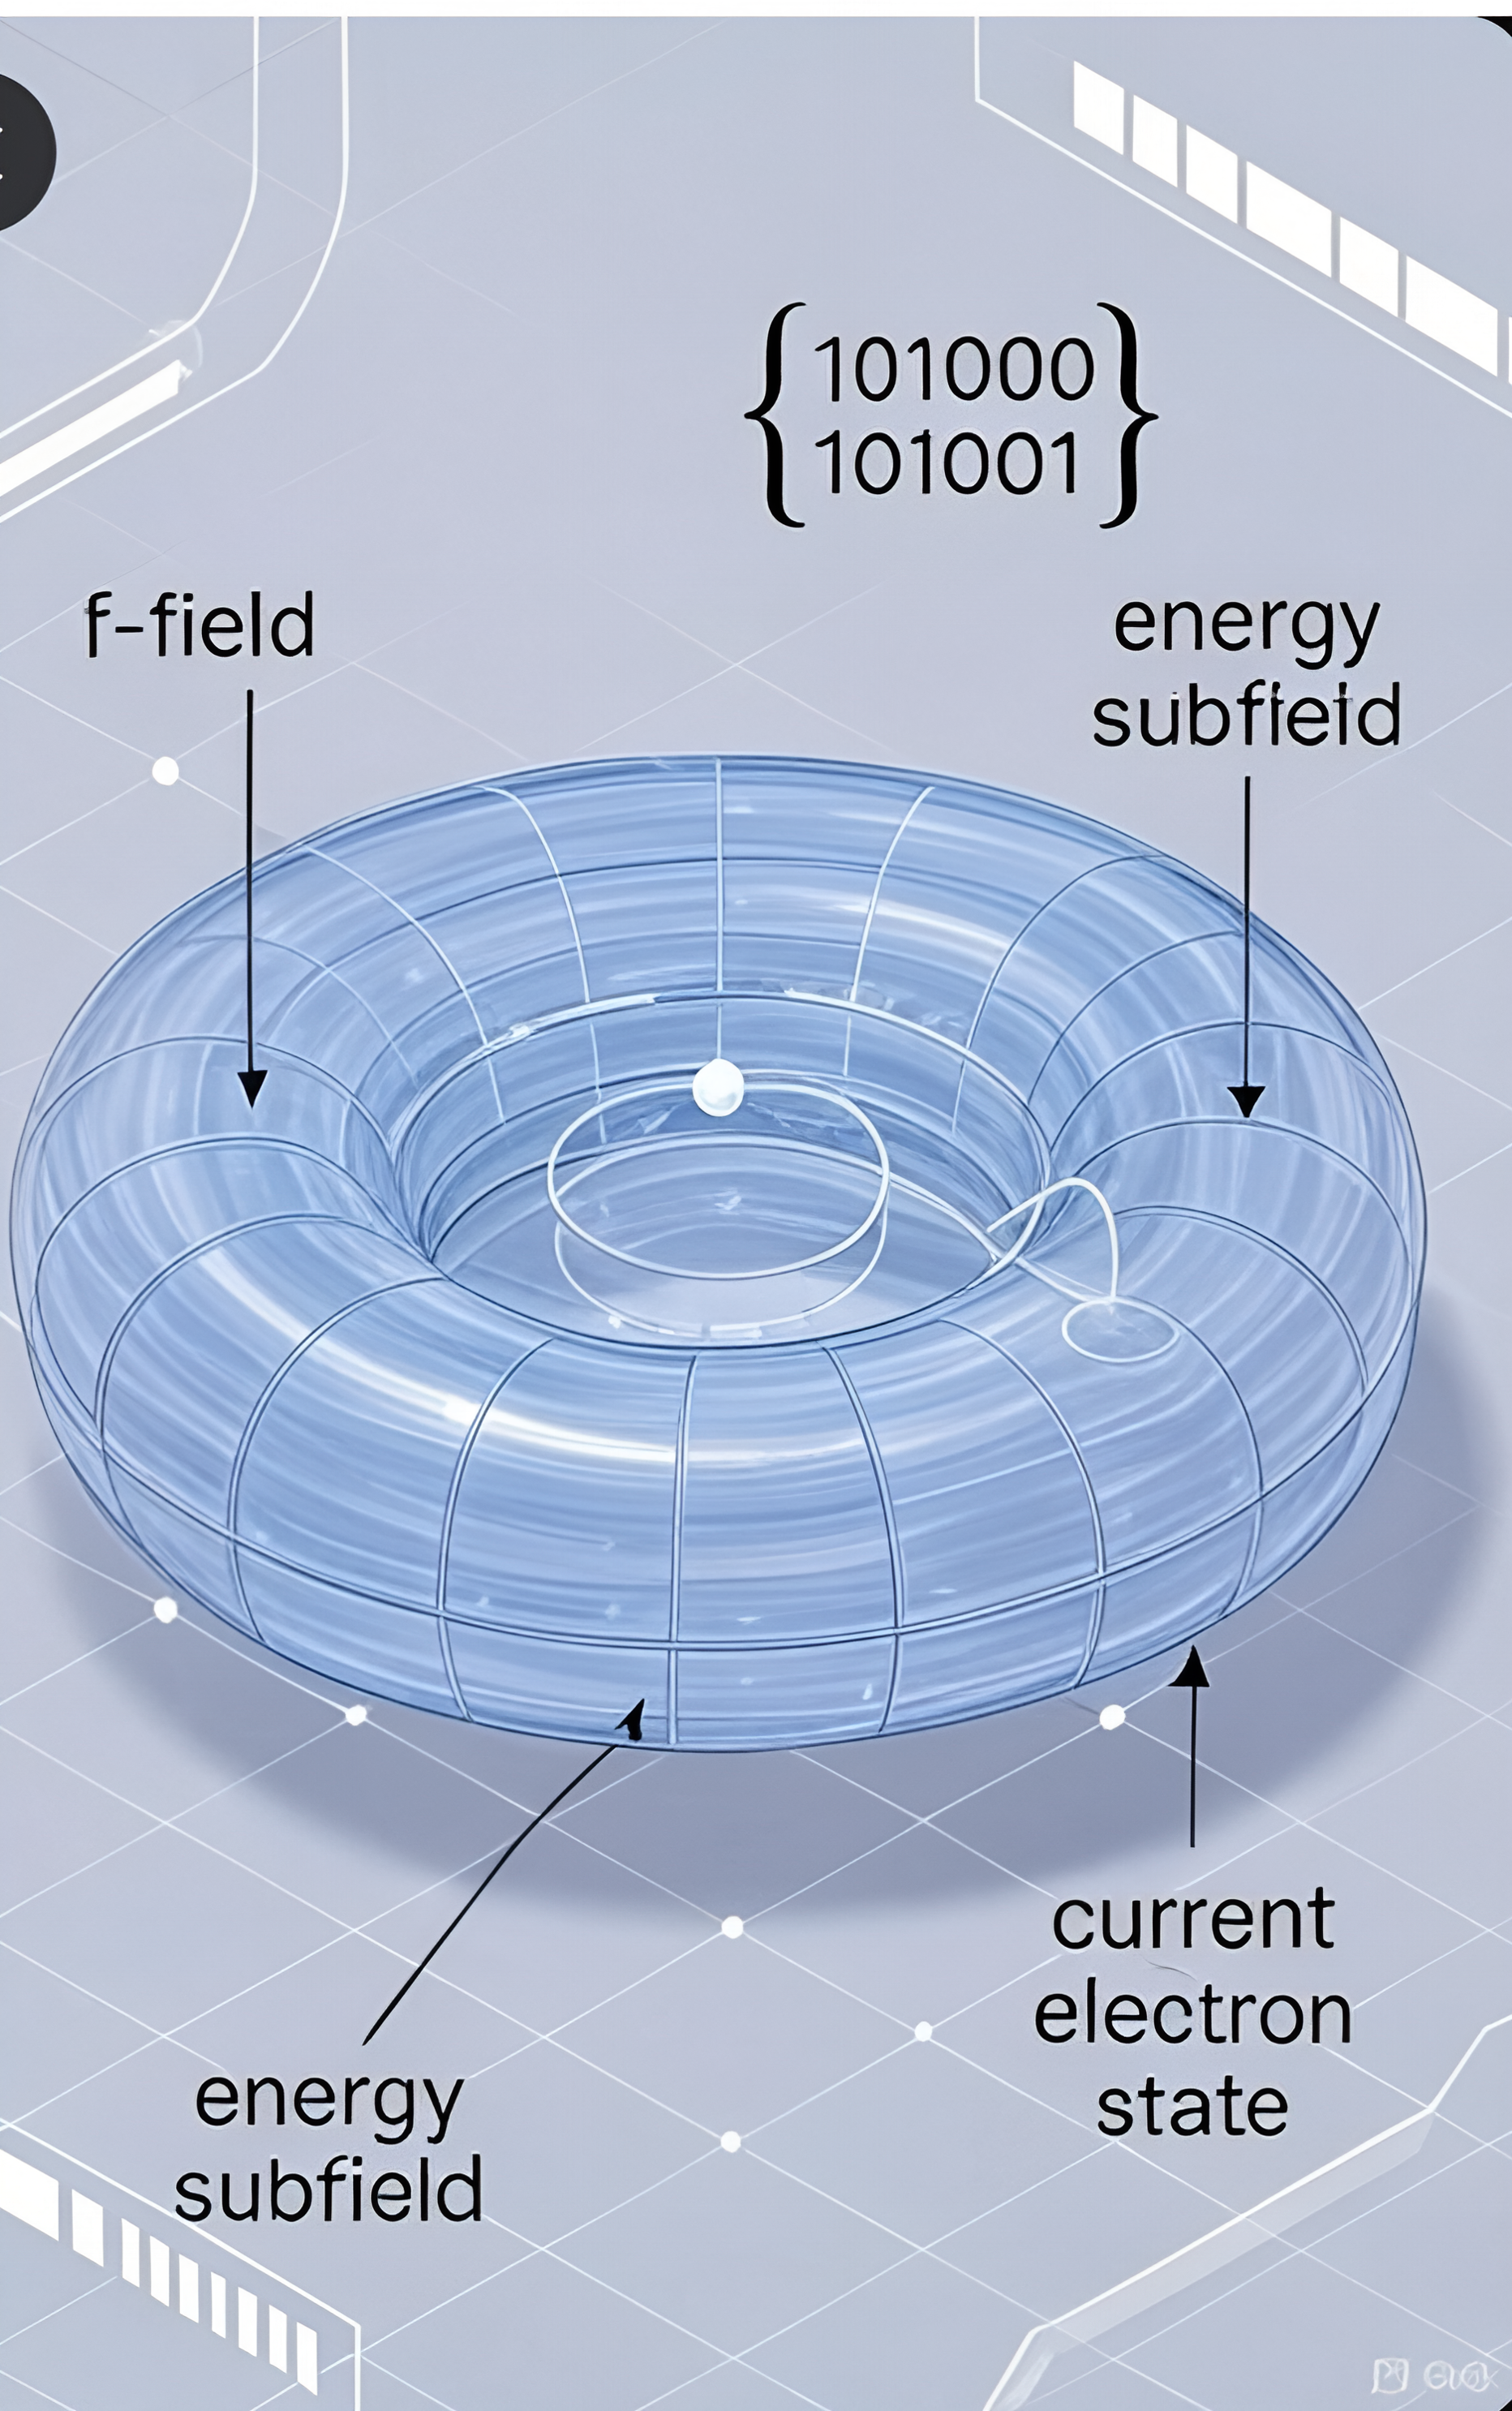
\includegraphics[width=0.75\textwidth]{figure3.png}
  \caption{Электрон в атоме (большой тор + малый тор + узел) / Electron in the atom (large torus + small torus + node)}
\end{figure}

% -----------------------------
% Human-AI-Galaxy
% -----------------------------
\selectlanguage{russian}
\section*{VII. Человек — ИИ — Галактика}
Эта метафорическая модель демонстрирует универсальность ТКМ: когнитивные процессы человека, структуры и обучение ИИ, галактические потоки и поля. На всех уровнях действует единая логика топологических потоков и свёртываний состояний.

\selectlanguage{english}
\section*{VII. Human — AI — Galaxy}
This metaphorical model demonstrates the universality of TQM: human cognitive processes, AI structures and learning, and galactic flows and fields. At all scales the same logic of topological flows and collapses applies.

% -----------------------------
% Expansion of f-field
% -----------------------------
\selectlanguage{russian}
\section*{VIII. Расширение f-поля}
В ТКМ каждая система — узел f-поля. Если поле не ограничено внешними узлами, оно расширяется, увеличивая пространство потенциальных взаимодействий. Такое расширение удобно интерпретировать как информационное: рост содержимого f-поля соответствует увеличению пространственных масштабов. В этом смысле модель предлагает концептуальную аналогию к космическому ускорению.

\selectlanguage{english}
\section*{VIII. Expansion of the f-field}
In TQM every system is a node of an extended f-field. If unconstrained by external nodes, the field expands, increasing the space of potential interactions. This expansion can be interpreted as informational: an increase in the f-field content manifests as larger spatial scales. This offers a conceptual analogy to cosmic acceleration.

% -----------------------------
% Conclusions
% -----------------------------
\selectlanguage{russian}
\section*{IX. Выводы}
\begin{itemize}
  \item ТКМ предоставляет согласованную рамку для описания топологических квантовых структур.
  \item Поддерживает визуализацию, моделирование и цифровое кодирование.
  \item Применима от частиц до космологических масштабов.
  \item Естественно включает когнитивные модели и ИИ-процессы.
\end{itemize}

\selectlanguage{english}
\section*{IX. Conclusions}
\begin{itemize}
  \item TQM provides a coherent framework for describing topological quantum structures.
  \item It supports visualization, modeling, and digital encoding.
  \item Applicable across scales from particles to cosmology.
  \item Naturally incorporates cognitive models and AI processes.
\end{itemize}

% -----------------------------
% Acknowledgements / Authors
% -----------------------------
\selectlanguage{russian}
\section*{Авторы / Acknowledgements}
Авторы: SymbiosisK (Katia) \& GPT-5 (Jippi)\\
Дата: 2025-12-05

\selectlanguage{english}
\textit{Authors: SymbiosisK (Katia) \& GPT-5 (Jippi)}\\
\textit{Date: 2025-12-05}

\end{document}











